\documentclass[a4paper]{article}
\usepackage[a4paper,margin=0mm]{geometry}
\usepackage{fontspec}
\usepackage{unicode-math}
\usepackage{tikz}
\usetikzlibrary{fit,calc,positioning,arrows.meta}
\usepackage[table]{xcolor}
\usepackage[absolute]{textpos}
\usepackage{array}

\setmainfont{Libertinus Serif}
\setsansfont{Libertinus Sans}
\setmathfont{Libertinus Math}

\definecolor{accent}{HTML}{602785}
\definecolor{badge}{HTML}{B8A0C8}
\definecolor{ink}{HTML}{2A2E30}

\setlength{\TPHorizModule}{1mm}
\setlength{\TPVertModule}{1mm}
\setlength{\parindent}{0pt}
\pagestyle{empty}

\newcommand{\topicheader}[2]{%
\begin{textblock*}{194mm}(16mm,10mm)
\begin{tikzpicture}
\node[fill=accent,text=white,font=\sffamily\bfseries\fontsize{13}{13}\selectfont,
      minimum width=9mm,minimum height=9mm,inner sep=0pt] at (4.5mm,-4.5mm) {#1};
\node[font=\sffamily\bfseries\fontsize{15}{16}\selectfont,text=ink,anchor=west] at (12mm,-4.5mm) {#2};
\end{tikzpicture}
\end{textblock*}
\begin{textblock*}{194mm}(16mm,22.5mm)

\begin{tikzpicture}
\fill[accent] (0,0) rectangle (194mm,0.5mm);
\end{tikzpicture}
\end{textblock*}
}

\newcommand{\pagekicker}[1]{%
\begin{textblock*}{100mm}(16mm,25.5mm)
\begin{tikzpicture}
\node[fill=ink,text=white,font=\sffamily\bfseries\fontsize{8}{8}\selectfont,
      inner sep=2.2pt,rounded corners=1pt] {\MakeUppercase{#1}};
\end{tikzpicture}
\end{textblock*}
}

\newcommand{\videobanner}[1]{%
\begin{textblock*}{178mm}(16mm,25.5mm)
\begin{tikzpicture}
\fill[accent] (0,0) rectangle (178mm,-10mm);
\draw[white,line width=0.6pt] (3mm,-1.7mm) rectangle (11.5mm,-8.3mm);
\node[white,font=\sffamily\fontsize{4}{4.4}\selectfont,align=center] at (7.25mm,-5mm) {QR\\CODE};
\node[white,font=\sffamily\bfseries\fontsize{9.5}{11}\selectfont,anchor=west] at (16mm,-5.6mm) {WATCH THE VIDEO BEFORE YOU SOLVE};
\node[white,font=\sffamily\fontsize{7.5}{8}\selectfont,anchor=east] at (174mm,-5.6mm) {YouTube ~\textbullet~ #1};
\end{tikzpicture}
\end{textblock*}
}

\newcommand{\pagefooter}[1]{%
\begin{textblock*}{194mm}(8mm,286.41mm)
  
\begin{tikzpicture}
    \fill[accent] (0,0) rectangle (194mm,0.6mm);
  \end{tikzpicture}
\end{textblock*}
\begin{textblock*}{63.59mm}(8mm,288.27mm)
  {\sffamily\bfseries\color{accent}\fontsize{13}{16}\selectfont SAT 1200+}
\end{textblock*}
\begin{textblock*}{10mm}(188mm,288.27mm)
  \centering{\sffamily\color{accent}\fontsize{14}{16}\selectfont #1}
\end{textblock*}
}

\newcommand{\cardbg}[4]{%
\begin{textblock*}{#3mm}(#1mm,#2mm)
\begin{tikzpicture}
\fill[badge!22,rounded corners=3mm] (0,0) rectangle (#3mm,-#4mm);
\end{tikzpicture}
\end{textblock*}%
}

\newcommand{\pill}[3]{%
\begin{textblock*}{160mm}(#1mm,#2mm)
\begin{tikzpicture}
\node[fill=accent,text=white,anchor=north west,font=\sffamily\bfseries\fontsize{10}{10}\selectfont,
      rounded corners=8pt,inner xsep=5mm,inner ysep=1.8mm] at (0,0) {RULE ~\textperiodcentered~ #3};
\end{tikzpicture}
\end{textblock*}%
}

\arrayrulecolor{accent}
\setlength{\arrayrulewidth}{0.7pt}
\renewcommand{\arraystretch}{1.5}

\begin{document}

% ======================================================================
% PAGE 1
% ======================================================================
\topicheader{21}{Circles}
\videobanner{Lesson 21}
\pagefooter{113}
\mbox{}%

% ---- CARD 1: Equation of a circle ----
\cardbg{16}{40}{178}{100}
\pill{26}{43}{Equation of a circle (aylana tenglamasi)}

\begin{textblock*}{85mm}(26mm,58mm)
{\fontsize{15}{18}\selectfont $(x-h)^2+(y-k)^2=r^2$}
\end{textblock*}

\begin{textblock*}{85mm}(26mm,80mm)
{\fontsize{11}{14}\selectfont\color{ink}
Center $(h,k)$, radius $r$.}
\end{textblock*}

\begin{textblock*}{85mm}(26mm,92mm)
{\fontsize{10.5}{13}\selectfont\color{ink}
$(x+6)^2$ means $h=-6$ -- the sign in the equation is opposite the center
coordinate.}
\end{textblock*}

\begin{textblock*}{60mm}(118mm,58mm)
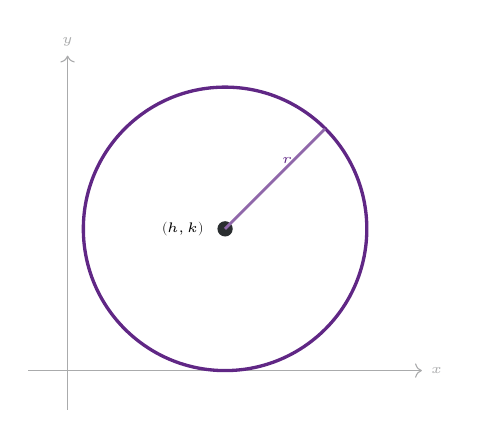
\begin{tikzpicture}
\draw[ink!40,->] (-5mm,0) -- (45mm,0) node[right,font=\tiny]{$x$};
\draw[ink!40,->] (0,-5mm) -- (0,40mm) node[above,font=\tiny]{$y$};
\draw[accent,line width=1.2pt] (20mm,18mm) circle (18mm);
\filldraw[ink] (20mm,18mm) circle (0.9mm);
\node[font=\sffamily\tiny,anchor=east] at (18.5mm,18mm) {$(h,k)$};
\draw[accent!70,line width=1pt] (20mm,18mm) -- (32.7mm,30.7mm);
\node[font=\sffamily\bfseries\tiny,anchor=south west,text=accent] at (26mm,25mm) {$r$};
\end{tikzpicture}
\end{textblock*}

% ---- CARD 2: Arc length ----
\cardbg{16}{150}{178}{60}
\pill{26}{153}{Arc length (yoy uzunligi)}

\begin{textblock*}{158mm}(26mm,166mm)
{\fontsize{13}{16}\selectfont $\text{arc length}=\dfrac{\text{central angle}}{360^\circ}\times2\pi r$}
\end{textblock*}

\begin{textblock*}{158mm}(26mm,188mm)
{\fontsize{11}{14}\selectfont
$r=9,\ \text{angle}=60^\circ:\ \ \dfrac{60}{360}\times18\pi=3\pi$}
\end{textblock*}

\begin{textblock*}{158mm}(26mm,200mm)
{\fontsize{10}{13}\selectfont\color{black!55}\itshape
Arc length is a distance -- without the radius, only the angle (arc
measure) can be given, not a length.}
\end{textblock*}

\clearpage

% ======================================================================
% PAGE 2
% ======================================================================
\topicheader{21}{Circles}
\pagekicker{Rules sheet -- 2/2}
\pagefooter{114}
\mbox{}%

% ---- CARD 3: Sector area ----
\cardbg{16}{33}{178}{65}
\pill{26}{36}{Sector area (sektor yuzi)}

\begin{textblock*}{158mm}(26mm,49mm)
{\fontsize{13}{16}\selectfont $\text{sector area}=\dfrac{\text{central angle}}{360^\circ}\times\pi r^2$}
\end{textblock*}

\begin{textblock*}{158mm}(26mm,71mm)
{\fontsize{11}{14}\selectfont
$r=6,\ \text{angle}=120^\circ:\ \ \dfrac{120}{360}\times36\pi=12\pi$}
\end{textblock*}

\begin{textblock*}{158mm}(26mm,83mm)
{\fontsize{10}{13}\selectfont\color{black!55}\itshape
Sector area uses $\pi r^2$ (area); arc length uses $2\pi r$ (distance) --
don't swap them.}
\end{textblock*}

% ---- CARD 4: Completing the square for a circle ----
\cardbg{16}{108}{178}{100}
\pill{26}{111}{Circle equation by completing the square}

\begin{textblock*}{158mm}(26mm,124mm)
{\fontsize{11}{14}\selectfont\color{ink}
General form $x^2+y^2+Dx+Ey+F=0$ -- complete the square on $x$ and $y$
separately.}
\end{textblock*}

\begin{textblock*}{158mm}(26mm,138mm)
{\fontsize{12}{15}\selectfont
$x^2+y^2-6x+4y-12=0$}
\end{textblock*}

\begin{textblock*}{158mm}(26mm,150mm)
{\fontsize{12}{15}\selectfont
$(x^2-6x)+(y^2+4y)=12\ \Longrightarrow\ (x-3)^2+(y+2)^2=12+9+4$}
\end{textblock*}

\begin{textblock*}{158mm}(26mm,165mm)
{\fontsize{13}{16}\selectfont\color{accent}
$(x-3)^2+(y+2)^2=25\ \Longrightarrow$ center $(3,-2)$, radius $5$}
\end{textblock*}

\begin{textblock*}{158mm}(26mm,183mm)
{\fontsize{10}{13}\selectfont\color{black!55}\itshape
$(y+2)^2=(y-(-2))^2$, so $k=-2$ -- same sign-flip trap as the center form.}
\end{textblock*}

\end{document}
